\documentclass{article}
\usepackage{graphicx}

\title{The Parallel Postulate}
\author{Joyce Huang}

\begin{document}

\maketitle
\begin{center}
    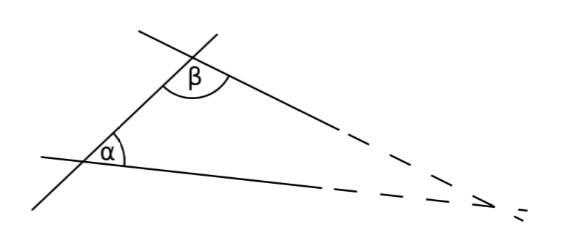
\includegraphics[scale = 0.5]{images/parallel1.png}
\end{center}
Of the five postulates that shoulder the entire subject of Euclidean geometry, one postulate stands out from the rest. In his fifth and final postulate, Euclid asserts that 

\begin{quote}
``If a line segment intersects two straight lines forming two interior angles on the same side that are less than two right angles, then the two lines, if extended indefinitely, meet on that side on which the angles sum to less than two right angles."
\end{quote}

A simpler version of the parallel postulate that is completely logically equivalent was postulated by John Playfair, called Playfair’s axiom:

\begin{quote}
“In a plane, given a line and a point not on it, at most one line parallel to the given line can be drawn through the point.”
\end{quote}

Like the other four postulates, the parallel postulate is very intuitive, but cannot be proven. Mathematicians have attempted to, though, to no avail. Interestingly enough, however, unlike the other four postulates, the exclusion or substitution of the parallel postulate creates completely different yet equally interesting systems of geometry such as non-Euclidean geometry, and absolute geometry. 

Geometries in which all but the parallel postulate are satisfied are called non-Euclidean geometries, some examples of which are hyperbolic geometry and elliptic geometry, which each result from a different alternate fifth postulate. 

\begin{center}
    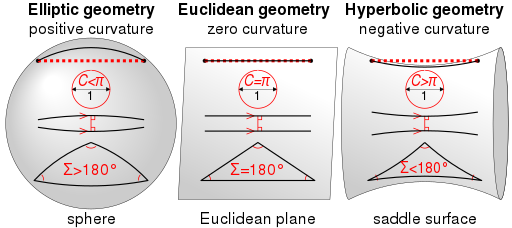
\includegraphics[scale = 0.3]{images/parallel3.png}
\end{center}

Geometry in which the first four postulates are satisfied and the parallel postulate and all its alternatives are excluded is called absolute geometry, which is also sometimes called neutral geometry. Absolute geometry is an \textit{incomplete axiomatic system}: with only four axioms, a fifth, independent axiom can be added without creating inconsistencies to form the basis for some Euclidean and non-Euclidean geometries. 

In the end, the first four of Euclid’s postulates are indisputable; they hold true in every realm of geometry discovered thus far. Meanwhile, the fifth postulate can be replaced with various different postulates to create the many different areas of geometry. For something so supposedly trivial, the parallel postulate is surprisingly disruptive.
\end{document}